\chapter{Predição de sucesso utilizando a nota de avaliação do IMDB}

A hipótese a ser analisada no processo pode ser descrita como: "para cada nó, é possível predizer sua nota com base nas notas dos vizinhos (ou seja, aqueles que atuaram com ele em algum momento)?". Em um teste inicial de viabilidade, verifica-se uma alta correlação entre a nota do ator e a média dos vizinhos utilizando a correlação de Pearson. O cálculo apontou uma correlação de 0,96 entre o conjunto de valores de notas dos vértices e a média das notas dos seus vizinhos imediatos. Essa alta correlação é consequência também da formação dos cliques, já que o vértice possui muitos vizinhos imediatos com uma nota próxima (ainda ponderado pela quantidade de elementos da vizinhança).

Utilizando a média como forma direta de predição, e comparando com a nota efetiva, é possível obter uma estimativa da acurácia. Neste caso, como forma de avaliação, é calculado o erro quadrático entre o valor predito e o real, e para toda a rede, obtém-se o erro médio. Neste caso, o erro médio obtido foi de 0,25 em notas que variam de 0 a 10. Ainda que o erro seja baixo, uma opção de modelo para predição é utilizar os conjuntos de valores para definir uma função linear que possa predizer melhor a nota com base na média. 

\begin{figure}[!htb]
\centering
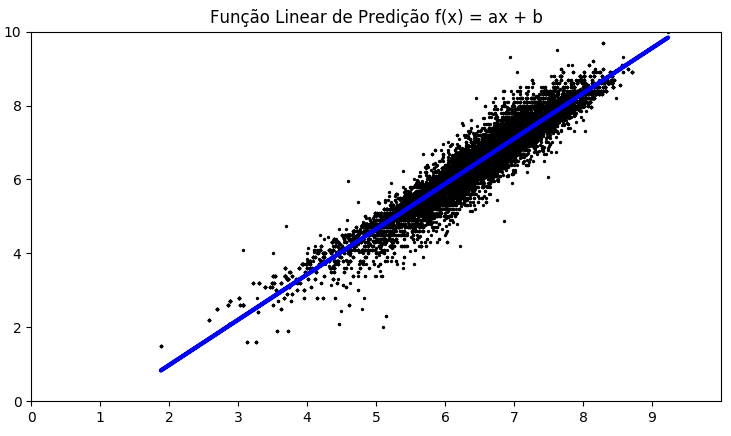
\includegraphics[width=15cm]{img/funcaolinear.png}
\caption{Função linear para melhor aproximação do conjunto de dados}
\label{fig:funcaolinear}
\end{figure}

A figura \ref{fig:funcaolinear} ilustra a dispersão dos valores e a reta que melhor estima os valores. Utilizando regressão linear, a função linear de variável simples que descreve essa reta é dada por f(x) = 1.22x - 1.47. Utilizando essa função para fazer a predição, o erro médio cai para 0,21(...). 
Indo um pouco além, outra hipótese é considerar um modelo multi-variável que considere as médias de vizinhos a distâncias N do vértice. Por exemplo, para N=2, a média dos vizinhos dos vizinhos também são consideradas para tentar ajustar melhor o modelo. Efetuando o primeiro teste para modelo multi-variável com N=2, obteve-se a função f(x) = 1.29x\textsubscript{1} + - 0.26x\textsubscript{2} - 0.19 (onde x\textsubscript{1} é a média dos vizinhos diretos, enquanto x\textsubscript{2} é a média dos vizinhos dos vizinhos). No entando, ao efetuar o teste de predição, o erro médio obtido foi da mesma ordem de 0.21(...), não justificando seu custo computacional.

Utilizando então a função linear obtida para predição, é possível tomar o seguinte cenário hipotético para ilustrar: um ator X, não conhecido previamente, mas que se sabe que atuou com Will Smith, Adam Sandler, Mila Kunis, Keanu Reeves, Rodrigo Santoro e Carrie Fisher (ilustrado na figura \ref{fig:predict}. O valor predito da sua média é obtido substituindo a variável na função pela média desses vizinhos. Esse valor seria dado então por 1,22 * 6,31 - 1,47 = 6,23.


\begin{figure}[!htb]
\centering
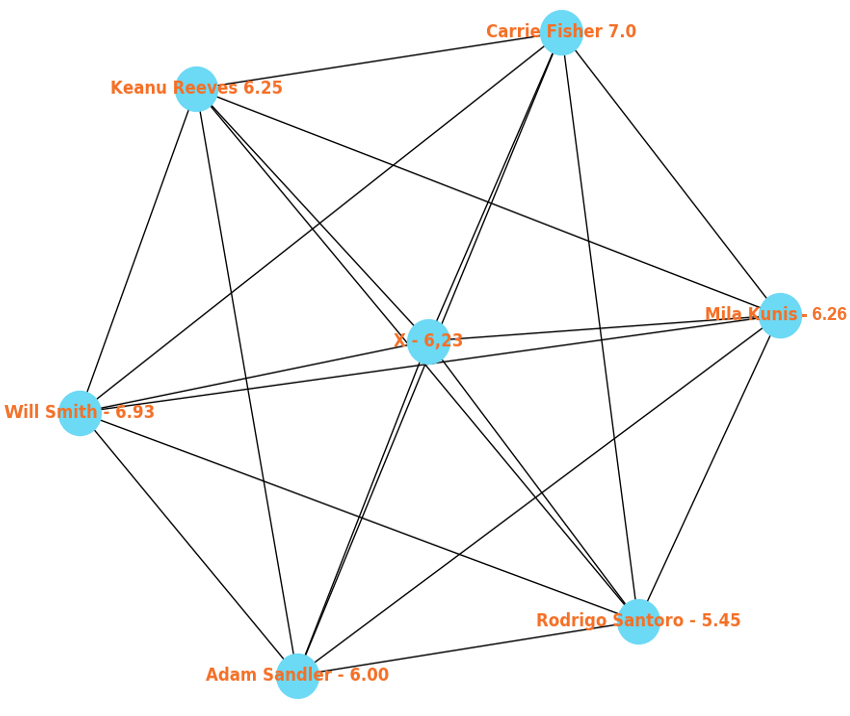
\includegraphics[width=16cm]{img/predict.png}
\caption{Cenário utilizando na predição}
\label{fig:predict}
\end{figure}
